\documentclass[slovene,11pt,a4paper]{article}
\usepackage[margin=1.8cm,bottom=3cm,foot=1.5cm]{geometry}
\usepackage{amsmath}
\usepackage{booktabs}
\usepackage{float}
\usepackage{graphicx}
\usepackage{gensymb}
\usepackage{geometry}
\usepackage{changepage}
\usepackage{subcaption}
\usepackage{multirow}
\usepackage{blindtext}
\usepackage{hyperref}
\usepackage[slovene]{babel}
\pagenumbering{gobble}
\renewcommand{\contentsname}{\centering Contents}

\begin{document}

\title{2. naloga - Linearno programiranje}
\author{Tadej Lozej 28201055}
\maketitle
\begin{center}
Modelska analiza 1 \\
\bigskip
Predavatelj: prof. dr. Simon Širca \\
Asistent: doc. dr. Miha Mihovilovič
\end{center}

\newpage

\tableofcontents

\newpage

\section{Uvod}

\pagenumbering{arabic}

V nalogi smo z uporabo linearnega programiranja sestavljali različne jedilnike. Iskali smo različne kombinacije živil iz tabele živil tako, da smo minimizirali določeno hranilo (kalorije, maščobe,...) ob nekih pogojih. Ti pogoji so bili maksimalen možen vnos hrane in minimalni dnevni vnos posameznega hranila. Na ta način smo sestavili več diet.

\section{Minimizacija kalorij}

Prva naloga je bila minimizacija kalorij pod pogojem, da zaužijemo zadostno količino posameznih hranil. Potrebne minimalne količine v našem jedilniku so $70\,$g maščob, $310\,$g ogljikovih hidratov, $50\,$g proteinov, $1000\,$mg kalcija, $18\,$mg železa, $60\,$mg vitamina C, $3500\,$mg kalija in od $500\,$mg do $2400\,$g natrija. Prav tako smo se omejili na maksimalno $2\,$kg zaužite hrane. Za zgled zapišimo naš problem kot

\[
\vec{c}\cdot \vec{x} = min, \quad A_{lb} \cdot \vec{x} \geq b_{lb}, \quad A_{ub} \cdot \vec{x} \leq b_{ub},
\]
kjer je $\vec{c}$ v tem primeru vektor vseh kaloričnih vrednosti živil, matriki $A_{lb}$ in $A_{ub}$ ter vektorja $b_{lb}$ in $b_{ub}$ ustrezni elementi s katerimi formuliramo pogoje o zadostnem vnosu posameznih hranil in maksimalno količino hrane, $\vec{x}$ pa iskani vektor, ki bo na $i$-tem mestu imel količino $i$-tega živila v dieti. Par $A_{lb}$ in $b_{lb}$ vsebuje pogoje o spodnjih mejah hranil. Sepravi o minimalnem dnevnem vnosu maščob, ogljikovih hidratov, proteinov... Par $A_{up}$ in $b_{up}$ pa pogoje o maksimalnem dnevnem vnosu natrija in maksimalnem dnevnem vnosu količine hrane.

Nalogo sem reševal v programskem jeziku Python in linearni problem minimizacije reševal s funkcijo \texttt{scipy.optimize.linprog}. Ta vedno minimizira produkt $\vec{c}\cdot \vec{x} =$ (če bi želeli iskati maksimum bi morali minimizirati $-\vec{c}\cdot \vec{x}$) in kot argument sprejme le matriko $A_{ub}$, zato moramo problem ustrezno preoblikovati. To storimo tako, da enačbo $\quad A_{lb} \cdot \vec{x} \geq b_{lb}$ pomožimo z $-1$, saj se v tem primeru neenačaj obrne.

Na sliki 1 lahko vidimo grafično predstavljen optimalen jedilnik problema minimizacije kalorij ob omenjenih pogojih. Na sliki 2 v tabeli vidimo rezultat naše minimizacije in hranilne vrednosti takšnega jedilnika. Vendar pri takem prehranjevanju zna priti do težav, saj več al manj zauživamo samo radensko in kakav. Želimo si bolj raznolike prehrane, zato postavimo nov pogoj.

\begin{figure}[h!]
  \centering
  \begin{minipage}[h]{0.56\textwidth}
    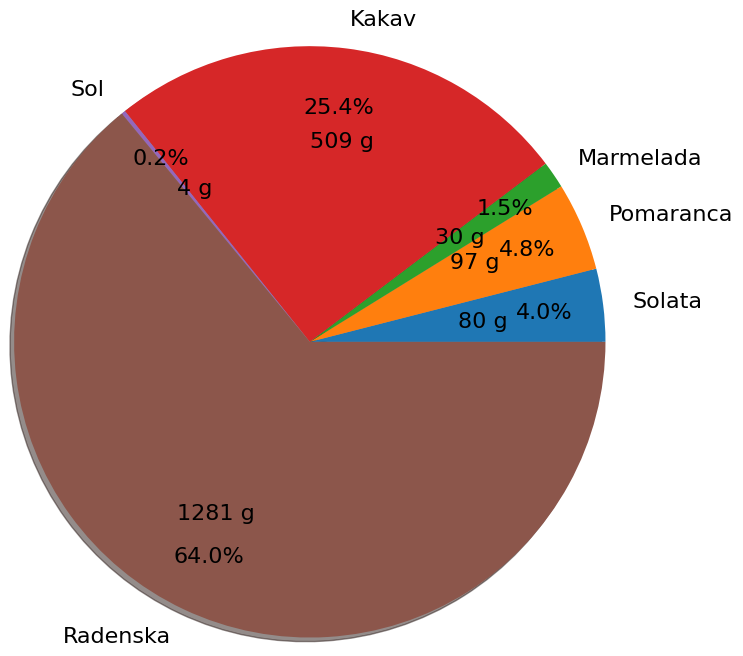
\includegraphics[width=\textwidth]{piechart1.png}
    \caption{Tortni diagram, ki prikazuje jedilnik z minimiziranimi kalorijami pri pogoju, da 				vsebuje dovolj hranil.}
  \end{minipage}
  \hfill
  \begin{minipage}[h]{0.42\textwidth}
	\begin{tabular}{lrr}
	  	\toprule
		{} &  Količina &  PDV[\%] \\
		\midrule
		energija[kcal]       &    1297.3 &         \\
		mascobe[g]           &      70.0 &   100.0 \\
		ogljikovi hidrati[g] &     310.0 &   100.0 \\
		proteini[g]          &     101.7 &   203.5 \\
		Ca[mg]               &    1000.0 &   100.0 \\
		Fe[mg]               &      72.6 &   403.5 \\
		Vitamin C[mg]        &      60.0 &   100.0 \\
		Kalij[mg]            &    8199.5 &   234.3 \\
		Natrij[mg]           &    2400.0 &   480.0 \\
		Cena[EUR]            &       4.2 &         \\
		\bottomrule
	\end{tabular}
	\caption{Tabela, ki prikazuje nutricijske vrednosti jedilnika na sliki 1.}
  \end{minipage}
\end{figure}

\newpage

Ker si želimo bolj raznolike prehrane je smiselno postaviti pogoj na količino posameznega živila. Recimo, da želimo konzumirati posameznega živila le do $200\,$g na dan. To storimo tako, da dovolimo le rešitve za $x\in(0,2)$. Še zmanjšamo prostor v katerem iščemo rešitve. V funkciji \texttt{scipy.optimize.linprog} to storimo preprosto z argumentom \texttt{bounds=(0,2)}. Dobimo jedilnik grafično in numerično predstavljen na slikah 3 in 4.

\begin{figure}[h!]
  \centering
  \begin{minipage}[h]{0.56\textwidth}
    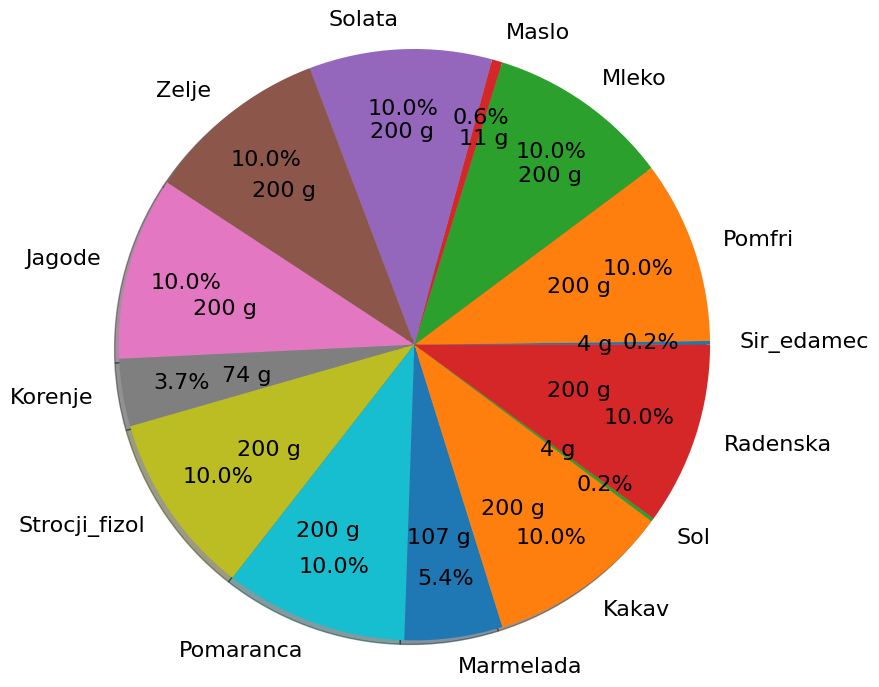
\includegraphics[width=\textwidth]{piechart2.png}
    \caption{Tortni diagram, ki prikazuje jedilnik z minimiziranimi kalorijami pri pogoju, da 				vsebuje dovolj hranil in z omejitvijo količine posameznega živila.}
  \end{minipage}
  \hfill
  \begin{minipage}[h]{0.42\textwidth}
	\begin{tabular}{lrr}
		\toprule
		{} &  Količina &  PDV[\%] \\
		\midrule
		energija[kcal]       &    1455.7 &         \\
		mascobe[g]           &      70.0 &   100.0 \\
		ogljikovi hidrati[g] &     310.0 &   100.0 \\
		proteini[g]          &      63.6 &   127.2 \\
		Ca[mg]               &    1000.0 &   100.0 \\
		Fe[mg]               &      34.8 &   193.3 \\
		Vitamin C[mg]        &     382.9 &   638.2 \\
		Kalij[mg]            &    6172.6 &   176.4 \\
		Natrij[mg]           &    2400.0 &   480.0 \\
		Cena[EUR]            &       6.0 &         \\
		\bottomrule
	\end{tabular}
	\caption{Tabela, ki prikazuje nutricijske vrednosti jedilnika na sliki 3.}
  \end{minipage}
\end{figure}

Drugi jedilnik je precej bolj raznolik kot prvi. To pomeni, da se je naš pogoj ustrezno poznal v praksi. Poleg radenske in kakava vidimo tukaj tudi precej sadja, zelenjave in tudi mlečne izdelke! Pri obeh jedilnikih vidimo, da so maščobe in ogljikovi hidrati na minimalni zahtevani vrednosti. To je dober znak, saj sta obe hranili kalorično najbogatejši med ostalimi.

\section{Minimizacija maščob}

Pogledali smo si jedilnik v katerem smo minimizirali kalorije. Sedaj sestavimo še jedilnik v katerem minimiziramo maščobe. V tem problemu sem odstranil pogoj o minimalnem vnosu maščob in dodal nov pogoj o minimalnem dnevnem vnosu kalorij $2000\,$kcal. Omejitev o maščobah sem odstranil, ker sem želel videti kakšna je najnižja vrednosti vnosa maščob pri pogoju, da zaužijemo zadostno količino drugih hranljivih snovi. Če bi spodnjo mejo za maščobe ohranili bi najverjetneje ta bila tudi rezultat, glede na to, da je bila tudi v prejšnjem jedilniku tudi, če tega nismo niti zahtevali. Vredno je omeniti, da sem omejitev količine posameznega živila upošteval tudi pri tem in vseh nadalnjih primerih.

Na sliki 5 lahko vidimo tortni diagram optimalnega jedilnika. Vanj so se prikradla živila, ki so energijsko bogata in imajo majhno vsebnost maščob kot na primer kruh, med in marmelada. Izključili smo vse mlečne izdelke in kakav, kljub njegovi bogati nutricijski vrednosti. Malo več kot polovico jedilnika sestavlja zgolj zelenjava (fizol, solata, zelje, brokoli...). na sliki 6 v tabeli vidimo, da smo maščobe minimizirali na $12,7\,$g. Ta vnos je približno petina priporočenega dnevnega vnosa, zato te diete na dolgi rok ne priporočam. Na spodnji zahtevani meji je vnos kalorij, kalcija in železa.

\newpage

\begin{figure}[h!]
  \centering
  \begin{minipage}[h]{0.56\textwidth}
    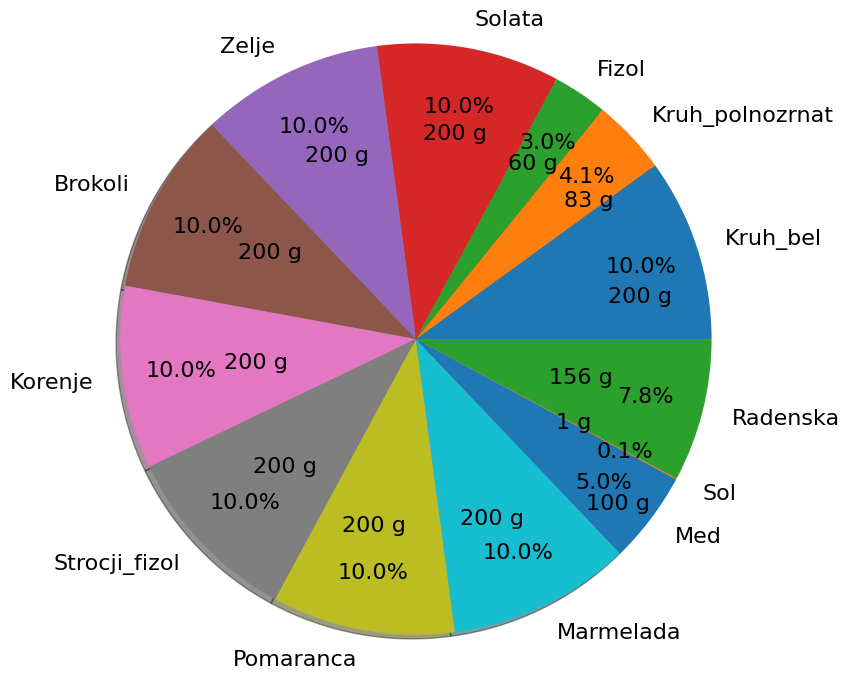
\includegraphics[width=\textwidth]{piechart3.png}
    \caption{Tortni diagram, ki prikazuje jedilnik z minimiziranimi maščobami pri pogoju, da 				vsebuje dovolj hranil in z omejitvijo količine posameznega živila.}
  \end{minipage}
  \hfill
  \begin{minipage}[h]{0.42\textwidth}
	\begin{tabular}{lrr}
		\toprule
		{} &  Količina &  PDV[\%] \\
		\midrule
		energija[kcal]       &    2000.0 &         \\
		mascobe[g]           &      12.7 &    18.1 \\
		ogljikovi hidrati[g] &     446.5 &   144.0 \\
		proteini[g]          &      56.8 &   113.6 \\
		Ca[mg]               &    1000.0 &   100.0 \\
		Fe[mg]               &      18.0 &   100.0 \\
		Vitamin C[mg]        &     430.9 &   718.2 \\
		Kalij[mg]            &    3703.2 &   105.8 \\
		Natrij[mg]           &    2400.0 &   480.0 \\
		Cena[EUR]            &       5.2 &         \\
		\bottomrule
	\end{tabular}
	\caption{Tabela, ki prikazuje nutricijske vrednosti jedilnika na sliki 5.}
  \end{minipage}
\end{figure}

\section{Minimizacija cene}

Še en primer minimizacije je minimizacija cene. Recimo, da želimo sestaviti jedilnik, ki vsebuje dovolj nutricijskih količin (v pogojih sem ohranil tudi minimalni vnos kalorij) in je najcenejši. Tortni diagram takšnega jedilnika prikazuje slika 7.

\begin{figure}[h!]
  \centering
  \begin{minipage}[h]{0.56\textwidth}
    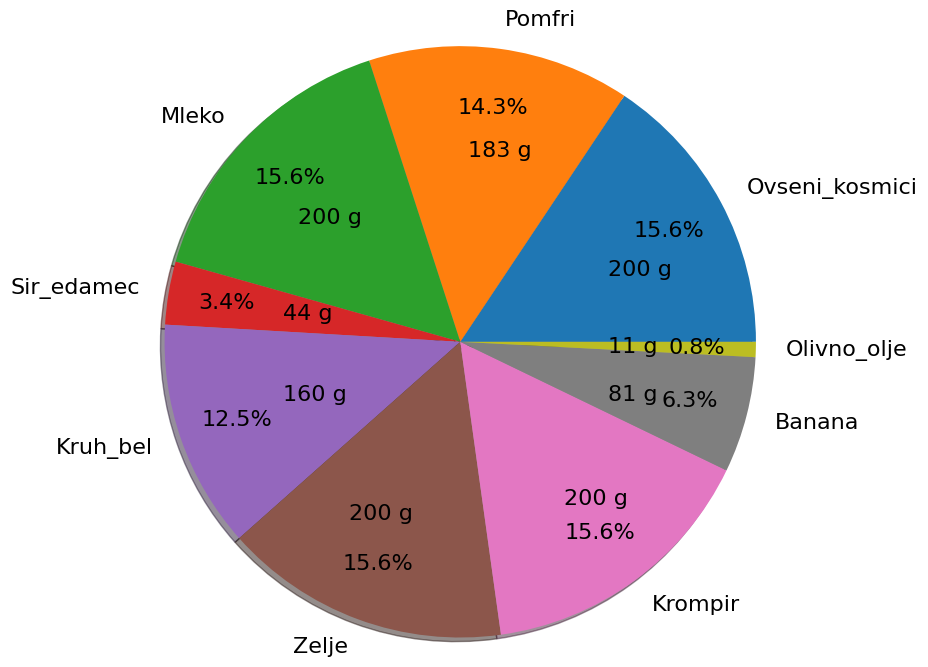
\includegraphics[width=\textwidth]{piechart4.png}
    \caption{Tortni diagram, ki prikazuje jedilnik z z minimizirano ceno pri pogoju, da 				vsebuje dovolj hranil in z omejitvijo količine posameznega živila.}
  \end{minipage}
  \hfill
  \begin{minipage}[h]{0.42\textwidth}
	\begin{tabular}{lrr}
		\toprule
		{} &  Količina &  PDV[\%] \\
		\midrule
		energija[kcal]       &    2000.0 &         \\
		mascobe[g]           &      70.0 &   100.0 \\
		ogljikovi hidrati[g] &     318.1 &   102.6 \\
		proteini[g]          &      77.1 &   154.2 \\
		Ca[mg]               &    1000.0 &   100.0 \\
		Fe[mg]               &      18.6 &   103.3 \\
		Vitamin C[mg]        &     143.4 &   239.1 \\
		Kalij[mg]            &    3500.0 &   100.0 \\
		Natrij[mg]           &    2400.0 &   480.0 \\
		Cena[EUR]            &       1.7 &         \\
		\bottomrule
	\end{tabular}
	\caption{Tabela, ki prikazuje nutricijske vrednosti jedilnika na sliki 7.}
  \end{minipage}
\end{figure}

Vidimo, da so vsa dobljena živila precej cenovno ugodna. Razen olivnega olja. Verjetno je to živilo prišlo zraven zato, ker smo z njim najlažje ustregli določenim pogojem (verjetno kalorije in maščobe). Na spodnji meji je poleg omenjenih hranil tudi kalij (najverjetneje banane). Za jedilnik pa odštejemo le $1,7\,$EUR.

\subsection{Minimizacija kalorij pri fiksni ceni}

Ko že govorimo o ceni, ki jo zapravljamo za jedilnik lahko omenim še kratko študijo, ki sem jo naredil. Na hitro sem raziskal kakovost jedilnika v odvisnosti od cene. Moral sem si izmisliti nek kvalifikator s katerim sem določil kakovost jedilnika. Odločil sem se za povprečni PDV hranil jedilnika. Tako sem minimiziral kalorije pri pogojih kot v drugem delu prvega poglavja in dodal pogoj o ceni jedilnika. To sem ponovil pri več različnih cenah in si beležil ceno, povprečni PDV hranil in kalorično vrednost jedilnika. Rezultate sem prikazal na grafu (slika 9). Vidimo, da se na grafu okrog cene $7,5\,$EUR pokaže nekakšen sweet spot za našo tabelo živil pri izbranih pogojih.

\begin{figure}[h!]
\centering
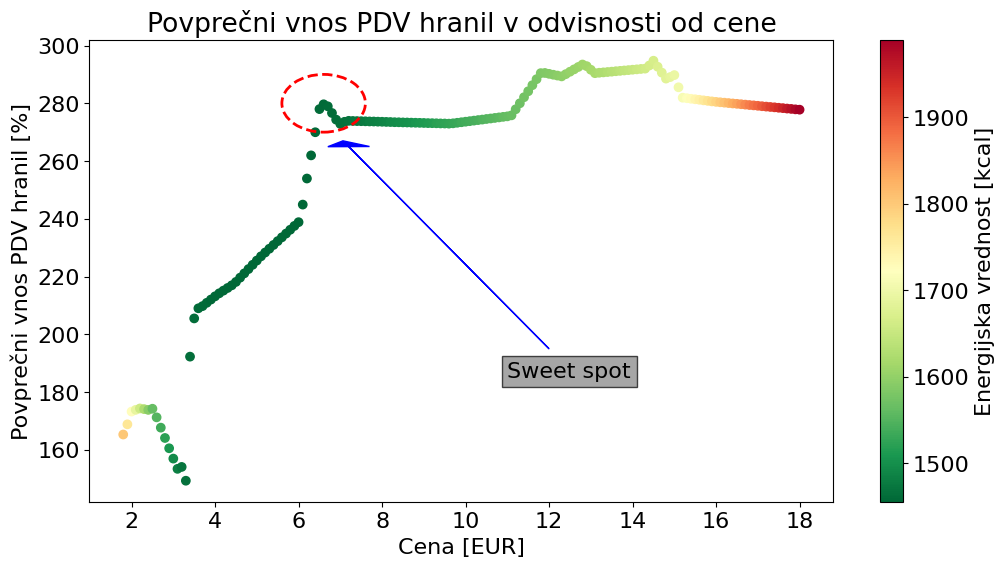
\includegraphics[width=14cm]{sweet.png}
\caption{Kakovost jedilnika in njegova kalorična vrednost v odvisnosti od cene. Na grafu vidimo očiten sweet spot za našo tabelo živil pri izbranih pogojih.}
\end{figure}

\section{Maksimizacija kalorij}

V poročilo sem želel dati tudi primer maksimizacije nečesa. Recimo, da ima eden izmed naših  otrok praznuje rojstnodnevno zabavo. Gostje so vabljeni takoj po zajtrku in zato moramo poskrbeti za celodnevni meni. Ker želimo, da bo zabava nepozabna moramo otrokom v jedilniku maksimizirati kalorije. Vseeno pa nočemo premašati mrzlih pogledov ostalih staršev in zato poskrbimo vsaj za zadostno količino posameznih hranil. Ker bolj zaupamo računalniškim algoritmom kot pa prehranskim svetovalcem se problema lotimo v Pythonu z linearnim programiranjem. Ta nam zastonj v sekundi vrne rezultate.

Na sliki 10 vidimo, da je jedilnik precej pester. Vsebuje vse od mesa in mlečnih izdelkov do sadja. Meni je pravzaprav super, saj hranila v njem vsebujejo velik odstotek PDV! Uspešno smo rešili problem in z nakupovalnim listkom ponosno odkorakamo v trgovino.

\newpage

\begin{figure}[h!]
  \centering
  \begin{minipage}[h]{0.56\textwidth}
    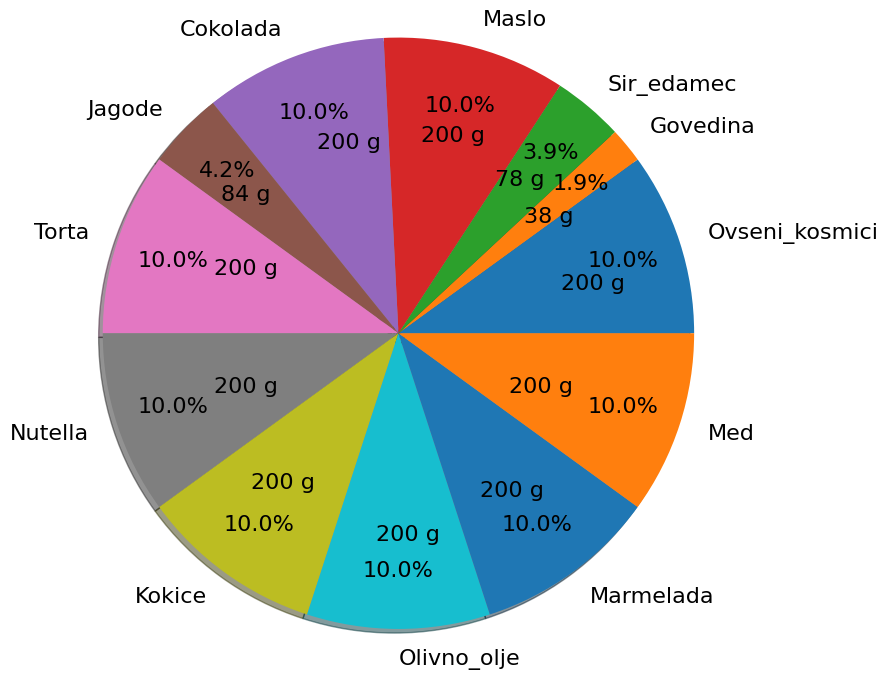
\includegraphics[width=\textwidth]{piechart5.png}
    \caption{Tortni diagram na katerem je prikazanih $200\,$g torte. Gre se za maksimizacijo kalorij ob pogojih minimalnega vnosa hranil.}
  \end{minipage}
  \hfill
  \begin{minipage}[h]{0.42\textwidth}
	\begin{tabular}{lrr}
		\toprule
		{} &  Količina &  PDV[\%] \\
		\midrule
		energija[kcal]       &    9205.4 &         \\
		mascobe[g]           &     573.7 &   819.6 \\
		ogljikovi hidrati[g] &     925.7 &   298.6 \\
		proteini[g]          &     120.4 &   240.9 \\
		Ca[mg]               &    1585.4 &   158.5 \\
		Fe[mg]               &      35.5 &   197.4 \\
		Vitamin C[mg]        &      60.0 &   100.0 \\
		Kalij[mg]            &    4369.7 &   124.8 \\
		Natrij[mg]           &    2400.0 &   480.0 \\
		Cena[EUR]            &      16.4 &         \\
		\bottomrule
		\end{tabular}
	\caption{Tabela, ki prikazuje nutricijske vrednosti $200\,$g torte v kombinaciji z drugimi živili na sliki 10.}
  \end{minipage}
\end{figure}

\section{Zaključek}

Na primeru smo se naučili uporabo linearnega programiranja. Gre za optimizacijo linearnih problemv z določenimi pogoji. Naloga mi je bila definitivno zanimiva in sem v njej užival.

\end{document}